\documentclass[1p]{elsarticle_modified}
%\bibliographystyle{elsarticle-num}

%\usepackage[colorlinks]{hyperref}
%\usepackage{abbrmath_seonhwa} %\Abb, \Ascr, \Acal ,\Abf, \Afrak
\usepackage{amsfonts}
\usepackage{amssymb}
\usepackage{amsmath}
\usepackage{amsthm}
\usepackage{scalefnt}
\usepackage{amsbsy}
\usepackage{kotex}
\usepackage{caption}
\usepackage{subfig}
\usepackage{color}
\usepackage{graphicx}
\usepackage{xcolor} %% white, black, red, green, blue, cyan, magenta, yellow
\usepackage{float}
\usepackage{setspace}
\usepackage{hyperref}

\usepackage{tikz}
\usetikzlibrary{arrows}

\usepackage{multirow}
\usepackage{array} % fixed length table
\usepackage{hhline}

%%%%%%%%%%%%%%%%%%%%%
\makeatletter
\renewcommand*\env@matrix[1][\arraystretch]{%
	\edef\arraystretch{#1}%
	\hskip -\arraycolsep
	\let\@ifnextchar\new@ifnextchar
	\array{*\c@MaxMatrixCols c}}
\makeatother %https://tex.stackexchange.com/questions/14071/how-can-i-increase-the-line-spacing-in-a-matrix
%%%%%%%%%%%%%%%

\usepackage[normalem]{ulem}

\newcommand{\msout}[1]{\ifmmode\text{\sout{\ensuremath{#1}}}\else\sout{#1}\fi}
%SOURCE: \msout is \stkout macro in https://tex.stackexchange.com/questions/20609/strikeout-in-math-mode

\newcommand{\cancel}[1]{
	\ifmmode
	{\color{red}\msout{#1}}
	\else
	{\color{red}\sout{#1}}
	\fi
}

\newcommand{\add}[1]{
	{\color{blue}\uwave{#1}}
}

\newcommand{\replace}[2]{
	\ifmmode
	{\color{red}\msout{#1}}{\color{blue}\uwave{#2}}
	\else
	{\color{red}\sout{#1}}{\color{blue}\uwave{#2}}
	\fi
}

\newcommand{\Sol}{\mathcal{S}} %segment
\newcommand{\D}{D} %diagram
\newcommand{\A}{\mathcal{A}} %arc


%%%%%%%%%%%%%%%%%%%%%%%%%%%%%5 test

\def\sl{\operatorname{\textup{SL}}(2,\Cbb)}
\def\psl{\operatorname{\textup{PSL}}(2,\Cbb)}
\def\quan{\mkern 1mu \triangleright \mkern 1mu}

\theoremstyle{definition}
\newtheorem{thm}{Theorem}[section]
\newtheorem{prop}[thm]{Proposition}
\newtheorem{lem}[thm]{Lemma}
\newtheorem{ques}[thm]{Question}
\newtheorem{cor}[thm]{Corollary}
\newtheorem{defn}[thm]{Definition}
\newtheorem{exam}[thm]{Example}
\newtheorem{rmk}[thm]{Remark}
\newtheorem{alg}[thm]{Algorithm}

\newcommand{\I}{\sqrt{-1}}
\begin{document}

%\begin{frontmatter}
%
%\title{Boundary parabolic representations of knots up to 8 crossings}
%
%%% Group authors per affiliation:
%\author{Yunhi Cho} 
%\address{Department of Mathematics, University of Seoul, Seoul, Korea}
%\ead{yhcho@uos.ac.kr}
%
%
%\author{Seonhwa Kim} %\fnref{s_kim}}
%\address{Center for Geometry and Physics, Institute for Basic Science, Pohang, 37673, Korea}
%\ead{ryeona17@ibs.re.kr}
%
%\author{Hyuk Kim}
%\address{Department of Mathematical Sciences, Seoul National University, Seoul 08826, Korea}
%\ead{hyukkim@snu.ac.kr}
%
%\author{Seokbeom Yoon}
%\address{Department of Mathematical Sciences, Seoul National University, Seoul, 08826,  Korea}
%\ead{sbyoon15@snu.ac.kr}
%
%\begin{abstract}
%We find all boundary parabolic representation of knots up to 8 crossings.
%
%\end{abstract}
%\begin{keyword}
%    \MSC[2010] 57M25 
%\end{keyword}
%
%\end{frontmatter}

%\linenumbers
%\tableofcontents
%
\newcommand\colored[1]{\textcolor{white}{\rule[-0.35ex]{0.8em}{1.4ex}}\kern-0.8em\color{red} #1}%
%\newcommand\colored[1]{\textcolor{white}{ #1}\kern-2.17ex	\textcolor{white}{ #1}\kern-1.81ex	\textcolor{white}{ #1}\kern-2.15ex\color{red}#1	}

{\Large $\underline{12a_{0563}~(K12a_{0563})}$}

\setlength{\tabcolsep}{10pt}
\renewcommand{\arraystretch}{1.6}
\vspace{1cm}\begin{tabular}{m{100pt}>{\centering\arraybackslash}m{274pt}}
\multirow{5}{120pt}{
	\centering
	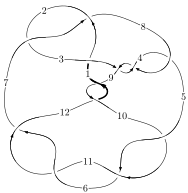
\includegraphics[width=112pt]{../../../GIT/diagram.site/Diagrams/png/1364_12a_0563.png}\\
\ \ \ A knot diagram\footnotemark}&
\allowdisplaybreaks
\textbf{Linearized knot diagam} \\
\cline{2-2}
 &
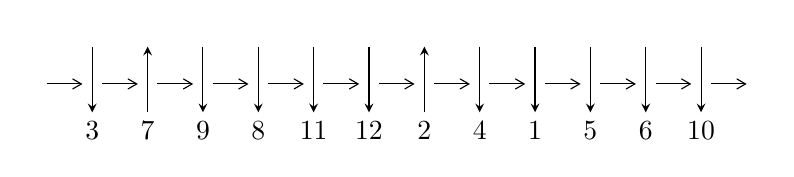
\begin{tikzpicture}[x=20pt, y=17pt]
	% nodes
	\node (C0) at (0, 0) {};
	\node (C1) at (1, 0) {};
	\node (C1U) at (1, +1) {};
	\node (C1D) at (1, -1) {3};

	\node (C2) at (2, 0) {};
	\node (C2U) at (2, +1) {};
	\node (C2D) at (2, -1) {7};

	\node (C3) at (3, 0) {};
	\node (C3U) at (3, +1) {};
	\node (C3D) at (3, -1) {9};

	\node (C4) at (4, 0) {};
	\node (C4U) at (4, +1) {};
	\node (C4D) at (4, -1) {8};

	\node (C5) at (5, 0) {};
	\node (C5U) at (5, +1) {};
	\node (C5D) at (5, -1) {11};

	\node (C6) at (6, 0) {};
	\node (C6U) at (6, +1) {};
	\node (C6D) at (6, -1) {12};

	\node (C7) at (7, 0) {};
	\node (C7U) at (7, +1) {};
	\node (C7D) at (7, -1) {2};

	\node (C8) at (8, 0) {};
	\node (C8U) at (8, +1) {};
	\node (C8D) at (8, -1) {4};

	\node (C9) at (9, 0) {};
	\node (C9U) at (9, +1) {};
	\node (C9D) at (9, -1) {1};

	\node (C10) at (10, 0) {};
	\node (C10U) at (10, +1) {};
	\node (C10D) at (10, -1) {5};

	\node (C11) at (11, 0) {};
	\node (C11U) at (11, +1) {};
	\node (C11D) at (11, -1) {6};

	\node (C12) at (12, 0) {};
	\node (C12U) at (12, +1) {};
	\node (C12D) at (12, -1) {10};
	\node (C13) at (13, 0) {};

	% arrows
	\draw[->,>={angle 60}]
	(C0) edge (C1) (C1) edge (C2) (C2) edge (C3) (C3) edge (C4) (C4) edge (C5) (C5) edge (C6) (C6) edge (C7) (C7) edge (C8) (C8) edge (C9) (C9) edge (C10) (C10) edge (C11) (C11) edge (C12) (C12) edge (C13) ;	\draw[->,>=stealth]
	(C1U) edge (C1D) (C2D) edge (C2U) (C3U) edge (C3D) (C4U) edge (C4D) (C5U) edge (C5D) (C6U) edge (C6D) (C7D) edge (C7U) (C8U) edge (C8D) (C9U) edge (C9D) (C10U) edge (C10D) (C11U) edge (C11D) (C12U) edge (C12D) ;
	\end{tikzpicture} \\
\hhline{~~} \\& 
\textbf{Solving Sequence} \\ \cline{2-2} 
 &
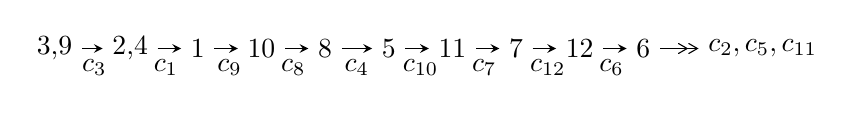
\begin{tikzpicture}[x=23pt, y=7pt]
	% node
	\node (A0) at (-1/8, 0) {3,9};
	\node (A1) at (17/16, 0) {2,4};
	\node (A2) at (17/8, 0) {1};
	\node (A3) at (25/8, 0) {10};
	\node (A4) at (33/8, 0) {8};
	\node (A5) at (41/8, 0) {5};
	\node (A6) at (49/8, 0) {11};
	\node (A7) at (57/8, 0) {7};
	\node (A8) at (65/8, 0) {12};
	\node (A9) at (73/8, 0) {6};
	\node (C1) at (1/2, -1) {$c_{3}$};
	\node (C2) at (13/8, -1) {$c_{1}$};
	\node (C3) at (21/8, -1) {$c_{9}$};
	\node (C4) at (29/8, -1) {$c_{8}$};
	\node (C5) at (37/8, -1) {$c_{4}$};
	\node (C6) at (45/8, -1) {$c_{10}$};
	\node (C7) at (53/8, -1) {$c_{7}$};
	\node (C8) at (61/8, -1) {$c_{12}$};
	\node (C9) at (69/8, -1) {$c_{6}$};
	\node (A10) at (11, 0) {$c_{2},c_{5},c_{11}$};

	% edge
	\draw[->,>=stealth]	
	(A0) edge (A1) (A1) edge (A2) (A2) edge (A3) (A3) edge (A4) (A4) edge (A5) (A5) edge (A6) (A6) edge (A7) (A7) edge (A8) (A8) edge (A9) ;
	\draw[->>,>={angle 60}]	
	(A9) edge (A10);
\end{tikzpicture} \\ 

\end{tabular} \\

\footnotetext{
The image of knot diagram is generated by the software ``\textbf{Draw programme}" developed by Andrew Bartholomew(\url{http://www.layer8.co.uk/maths/draw/index.htm\#Running-draw}), where we modified some parts for our purpose(\url{https://github.com/CATsTAILs/LinksPainter}).
}\phantom \\ \newline 
\centering \textbf{Ideals for irreducible components\footnotemark of $X_{\text{par}}$} 
 
\begin{align*}
I^u_{1}&=\langle 
-3.21428\times10^{21} u^{47}+3.07657\times10^{21} u^{46}+\cdots+1.91294\times10^{22} b+2.10944\times10^{22},\\
\phantom{I^u_{1}}&\phantom{= \langle  }8.01226\times10^{20} u^{47}-8.31592\times10^{20} u^{46}+\cdots+9.56472\times10^{20} a+3.53130\times10^{21},\;u^{48}- u^{47}+\cdots+u+2\rangle \\
I^u_{2}&=\langle 
- u^2+b,\;a-1,\;u^{18}+6 u^{16}+\cdots+u-1\rangle \\
I^u_{3}&=\langle 
b+1,\;a^4+a^3 u-4 a^3-3 a^2 u+5 a^2+3 a u-2 a- u+1,\;u^2+1\rangle \\
\\
\end{align*}
\raggedright * 3 irreducible components of $\dim_{\mathbb{C}}=0$, with total 74 representations.\\
\footnotetext{All coefficients of polynomials are rational numbers. But the coefficients are sometimes approximated in decimal forms when there is not enough margin.}
\newpage
\renewcommand{\arraystretch}{1}
\centering \section*{I. $I^u_{1}= \langle -3.21\times10^{21} u^{47}+3.08\times10^{21} u^{46}+\cdots+1.91\times10^{22} b+2.11\times10^{22},\;8.01\times10^{20} u^{47}-8.32\times10^{20} u^{46}+\cdots+9.56\times10^{20} a+3.53\times10^{21},\;u^{48}- u^{47}+\cdots+u+2 \rangle$}
\flushleft \textbf{(i) Arc colorings}\\
\begin{tabular}{m{7pt} m{180pt} m{7pt} m{180pt} }
\flushright $a_{3}=$&$\begin{pmatrix}1\\0\end{pmatrix}$ \\
\flushright $a_{9}=$&$\begin{pmatrix}0\\u\end{pmatrix}$ \\
\flushright $a_{2}=$&$\begin{pmatrix}-0.837689 u^{47}+0.869438 u^{46}+\cdots+13.2059 u-3.69201\\0.168028 u^{47}-0.160829 u^{46}+\cdots-1.56252 u-1.10272\end{pmatrix}$ \\
\flushright $a_{4}=$&$\begin{pmatrix}1\\u^2\end{pmatrix}$ \\
\flushright $a_{1}=$&$\begin{pmatrix}-0.669662 u^{47}+0.708609 u^{46}+\cdots+11.6434 u-4.79473\\0.168028 u^{47}-0.160829 u^{46}+\cdots-1.56252 u-1.10272\end{pmatrix}$ \\
\flushright $a_{10}=$&$\begin{pmatrix}-0.573968 u^{47}+0.0603230 u^{46}+\cdots+9.04562 u+5.11395\\0.0433537 u^{47}+0.0687272 u^{46}+\cdots-4.47263 u+1.08386\end{pmatrix}$ \\
\flushright $a_{8}=$&$\begin{pmatrix}u\\u^3+u\end{pmatrix}$ \\
\flushright $a_{5}=$&$\begin{pmatrix}u^2+1\\u^4+2 u^2\end{pmatrix}$ \\
\flushright $a_{11}=$&$\begin{pmatrix}-0.775286 u^{47}+0.102961 u^{46}+\cdots+16.4932 u+5.06341\\0.115161 u^{47}-0.190045 u^{46}+\cdots-4.11240 u+0.828323\end{pmatrix}$ \\
\flushright $a_{7}=$&$\begin{pmatrix}-0.519611 u^{47}+0.601722 u^{46}+\cdots+25.7485 u+2.68654\\-0.0513589 u^{47}-0.116669 u^{46}+\cdots-1.89721 u+1.51116\end{pmatrix}$ \\
\flushright $a_{12}=$&$\begin{pmatrix}-1.34327 u^{47}+1.07781 u^{46}+\cdots+27.0507 u+5.07361\\-0.273830 u^{47}+0.198143 u^{46}+\cdots+3.26013 u-0.158606\end{pmatrix}$ \\
\flushright $a_{6}=$&$\begin{pmatrix}1.33343 u^{47}-1.45372 u^{46}+\cdots-17.4102 u-8.92856\\0.00796109 u^{47}+0.0832675 u^{46}+\cdots-0.966904 u+0.230758\end{pmatrix}$\\&\end{tabular}
\flushleft \textbf{(ii) Obstruction class $= -1$}\\~\\
\flushleft \textbf{(iii) Cusp Shapes $= \frac{27465448057329986227}{27804404382329290780} u^{47}-\frac{1722649487279789829}{2780440438232929078} u^{46}+\cdots-\frac{776992786016705604511}{27804404382329290780} u-\frac{198347232390961135567}{13902202191164645390}$}\\~\\
\newpage\renewcommand{\arraystretch}{1}
\flushleft \textbf{(iv) u-Polynomials at the component}\newline \\
\begin{tabular}{m{50pt}|m{274pt}}
Crossings & \hspace{64pt}u-Polynomials at each crossing \\
\hline $$\begin{aligned}c_{1}\end{aligned}$$&$\begin{aligned}
&u^{48}+17 u^{47}+\cdots+35 u+4
\end{aligned}$\\
\hline $$\begin{aligned}c_{2},c_{7}\end{aligned}$$&$\begin{aligned}
&u^{48}+u^{47}+\cdots-3 u+2
\end{aligned}$\\
\hline $$\begin{aligned}c_{3},c_{4},c_{8}\end{aligned}$$&$\begin{aligned}
&u^{48}+u^{47}+\cdots- u+2
\end{aligned}$\\
\hline $$\begin{aligned}c_{5},c_{6},c_{10}\\c_{11}\end{aligned}$$&$\begin{aligned}
&u^{48}-2 u^{47}+\cdots+u+2
\end{aligned}$\\
\hline $$\begin{aligned}c_{9},c_{12}\end{aligned}$$&$\begin{aligned}
&u^{48}-8 u^{47}+\cdots-7639 u+1016
\end{aligned}$\\
\hline
\end{tabular}\\~\\
\newpage\renewcommand{\arraystretch}{1}
\flushleft \textbf{(v) Riley Polynomials at the component}\newline \\
\begin{tabular}{m{50pt}|m{274pt}}
Crossings & \hspace{64pt}Riley Polynomials at each crossing \\
\hline $$\begin{aligned}c_{1}\end{aligned}$$&$\begin{aligned}
&y^{48}+37 y^{47}+\cdots+12799 y+16
\end{aligned}$\\
\hline $$\begin{aligned}c_{2},c_{7}\end{aligned}$$&$\begin{aligned}
&y^{48}+17 y^{47}+\cdots+35 y+4
\end{aligned}$\\
\hline $$\begin{aligned}c_{3},c_{4},c_{8}\end{aligned}$$&$\begin{aligned}
&y^{48}+53 y^{47}+\cdots-237 y+4
\end{aligned}$\\
\hline $$\begin{aligned}c_{5},c_{6},c_{10}\\c_{11}\end{aligned}$$&$\begin{aligned}
&y^{48}-52 y^{47}+\cdots+19 y+4
\end{aligned}$\\
\hline $$\begin{aligned}c_{9},c_{12}\end{aligned}$$&$\begin{aligned}
&y^{48}+32 y^{47}+\cdots-318369 y+1032256
\end{aligned}$\\
\hline
\end{tabular}\\~\\
\newpage\flushleft \textbf{(vi) Complex Volumes and Cusp Shapes}
$$\begin{array}{c|c|c}  
\text{Solutions to }I^u_{1}& \I (\text{vol} + \sqrt{-1}CS) & \text{Cusp shape}\\
 \hline 
\begin{aligned}
u &= -0.279405 + 0.971105 I \\
a &= \phantom{-}0.633756 + 0.239746 I \\
b &= \phantom{-}0.165180 + 0.161172 I\end{aligned}
 & -4.68544 + 3.19221 I & -6.37639 - 4.16497 I \\ \hline\begin{aligned}
u &= -0.279405 - 0.971105 I \\
a &= \phantom{-}0.633756 - 0.239746 I \\
b &= \phantom{-}0.165180 - 0.161172 I\end{aligned}
 & -4.68544 - 3.19221 I & -6.37639 + 4.16497 I \\ \hline\begin{aligned}
u &= \phantom{-}0.881286 + 0.378029 I \\
a &= -0.468437 + 0.143230 I \\
b &= -0.67254 - 1.34172 I\end{aligned}
 & -5.10511 - 9.85415 I & -11.23414 + 7.48976 I \\ \hline\begin{aligned}
u &= \phantom{-}0.881286 - 0.378029 I \\
a &= -0.468437 - 0.143230 I \\
b &= -0.67254 + 1.34172 I\end{aligned}
 & -5.10511 + 9.85415 I & -11.23414 - 7.48976 I \\ \hline\begin{aligned}
u &= -0.845379 + 0.414724 I \\
a &= -0.399315 - 0.163435 I \\
b &= -0.586845 + 1.279740 I\end{aligned}
 & \phantom{-}1.89498 + 7.08453 I & -7.53014 - 8.63075 I \\ \hline\begin{aligned}
u &= -0.845379 - 0.414724 I \\
a &= -0.399315 + 0.163435 I \\
b &= -0.586845 - 1.279740 I\end{aligned}
 & \phantom{-}1.89498 - 7.08453 I & -7.53014 + 8.63075 I \\ \hline\begin{aligned}
u &= -0.757362 + 0.544501 I \\
a &= -0.177555 - 0.142317 I \\
b &= -0.315094 + 1.121340 I\end{aligned}
 & -3.80725 + 0.44416 I & -9.21656 - 2.62442 I \\ \hline\begin{aligned}
u &= -0.757362 - 0.544501 I \\
a &= -0.177555 + 0.142317 I \\
b &= -0.315094 - 1.121340 I\end{aligned}
 & -3.80725 - 0.44416 I & -9.21656 + 2.62442 I \\ \hline\begin{aligned}
u &= \phantom{-}0.801878 + 0.461107 I \\
a &= -0.308887 + 0.177382 I \\
b &= -0.484403 - 1.202350 I\end{aligned}
 & \phantom{-}2.31942 - 3.03168 I & -5.96588 + 2.35658 I \\ \hline\begin{aligned}
u &= \phantom{-}0.801878 - 0.461107 I \\
a &= -0.308887 - 0.177382 I \\
b &= -0.484403 + 1.202350 I\end{aligned}
 & \phantom{-}2.31942 + 3.03168 I & -5.96588 - 2.35658 I\\
 \hline 
 \end{array}$$\newpage$$\begin{array}{c|c|c}  
\text{Solutions to }I^u_{1}& \I (\text{vol} + \sqrt{-1}CS) & \text{Cusp shape}\\
 \hline 
\begin{aligned}
u &= \phantom{-}0.094584 + 0.916633 I \\
a &= \phantom{-}0.842564 - 0.081921 I \\
b &= -0.0039149 - 0.0498200 I\end{aligned}
 & \phantom{-}1.88453 - 1.52925 I & -1.27440 + 5.26025 I \\ \hline\begin{aligned}
u &= \phantom{-}0.094584 - 0.916633 I \\
a &= \phantom{-}0.842564 + 0.081921 I \\
b &= -0.0039149 + 0.0498200 I\end{aligned}
 & \phantom{-}1.88453 + 1.52925 I & -1.27440 - 5.26025 I \\ \hline\begin{aligned}
u &= \phantom{-}0.019449 + 1.296200 I \\
a &= \phantom{-}0.96626 + 1.66275 I \\
b &= -0.218022 - 0.686915 I\end{aligned}
 & -4.87695 + 2.29360 I & \phantom{-0.000000 } 0 \\ \hline\begin{aligned}
u &= \phantom{-}0.019449 - 1.296200 I \\
a &= \phantom{-}0.96626 - 1.66275 I \\
b &= -0.218022 + 0.686915 I\end{aligned}
 & -4.87695 - 2.29360 I & \phantom{-0.000000 } 0 \\ \hline\begin{aligned}
u &= \phantom{-}0.662333 + 0.127045 I \\
a &= -0.823194 + 0.695101 I \\
b &= -1.028930 - 0.838109 I\end{aligned}
 & -10.70200 - 3.57800 I & -16.9686 + 4.2625 I \\ \hline\begin{aligned}
u &= \phantom{-}0.662333 - 0.127045 I \\
a &= -0.823194 - 0.695101 I \\
b &= -1.028930 + 0.838109 I\end{aligned}
 & -10.70200 + 3.57800 I & -16.9686 - 4.2625 I \\ \hline\begin{aligned}
u &= -0.027632 + 1.374070 I \\
a &= \phantom{-}0.60190 - 1.62387 I \\
b &= -0.134767 + 0.924503 I\end{aligned}
 & \phantom{-}3.01436 - 0.56771 I & \phantom{-0.000000 } 0 \\ \hline\begin{aligned}
u &= -0.027632 - 1.374070 I \\
a &= \phantom{-}0.60190 + 1.62387 I \\
b &= -0.134767 - 0.924503 I\end{aligned}
 & \phantom{-}3.01436 + 0.56771 I & \phantom{-0.000000 } 0 \\ \hline\begin{aligned}
u &= \phantom{-}0.218315 + 1.358270 I \\
a &= \phantom{-}0.09353 + 2.15802 I \\
b &= -0.696041 - 1.142180 I\end{aligned}
 & -5.99306 - 6.70057 I & \phantom{-0.000000 } 0 \\ \hline\begin{aligned}
u &= \phantom{-}0.218315 - 1.358270 I \\
a &= \phantom{-}0.09353 - 2.15802 I \\
b &= -0.696041 + 1.142180 I\end{aligned}
 & -5.99306 + 6.70057 I & \phantom{-0.000000 } 0\\
 \hline 
 \end{array}$$\newpage$$\begin{array}{c|c|c}  
\text{Solutions to }I^u_{1}& \I (\text{vol} + \sqrt{-1}CS) & \text{Cusp shape}\\
 \hline 
\begin{aligned}
u &= -0.574563 + 0.232091 I \\
a &= -0.449839 - 0.845197 I \\
b &= -0.830134 + 0.745730 I\end{aligned}
 & -2.99542 + 2.92052 I & -16.1336 - 6.6064 I \\ \hline\begin{aligned}
u &= -0.574563 - 0.232091 I \\
a &= -0.449839 + 0.845197 I \\
b &= -0.830134 - 0.745730 I\end{aligned}
 & -2.99542 - 2.92052 I & -16.1336 + 6.6064 I \\ \hline\begin{aligned}
u &= -0.17592 + 1.40998 I \\
a &= \phantom{-}0.17221 - 1.93269 I \\
b &= -0.509228 + 1.232380 I\end{aligned}
 & \phantom{-}2.29935 + 5.57635 I & \phantom{-0.000000 } 0 \\ \hline\begin{aligned}
u &= -0.17592 - 1.40998 I \\
a &= \phantom{-}0.17221 + 1.93269 I \\
b &= -0.509228 - 1.232380 I\end{aligned}
 & \phantom{-}2.29935 - 5.57635 I & \phantom{-0.000000 } 0 \\ \hline\begin{aligned}
u &= \phantom{-}0.09301 + 1.43048 I \\
a &= \phantom{-}0.33273 + 1.72234 I \\
b &= -0.243029 - 1.177930 I\end{aligned}
 & \phantom{-}5.11959 - 2.66046 I & \phantom{-0.000000 } 0 \\ \hline\begin{aligned}
u &= \phantom{-}0.09301 - 1.43048 I \\
a &= \phantom{-}0.33273 - 1.72234 I \\
b &= -0.243029 + 1.177930 I\end{aligned}
 & \phantom{-}5.11959 + 2.66046 I & \phantom{-0.000000 } 0 \\ \hline\begin{aligned}
u &= \phantom{-}0.328252 + 0.355874 I \\
a &= \phantom{-}0.529736 + 1.011980 I \\
b &= -0.606974 - 0.412729 I\end{aligned}
 & -0.575619 - 1.189230 I & -7.30572 + 5.21199 I \\ \hline\begin{aligned}
u &= \phantom{-}0.328252 - 0.355874 I \\
a &= \phantom{-}0.529736 - 1.011980 I \\
b &= -0.606974 + 0.412729 I\end{aligned}
 & -0.575619 + 1.189230 I & -7.30572 - 5.21199 I \\ \hline\begin{aligned}
u &= \phantom{-}0.33907 + 1.49289 I \\
a &= -0.27071 + 1.81325 I \\
b &= -0.88608 - 1.67141 I\end{aligned}
 & \phantom{-}0.9224 - 14.2869 I & \phantom{-0.000000 } 0 \\ \hline\begin{aligned}
u &= \phantom{-}0.33907 - 1.49289 I \\
a &= -0.27071 - 1.81325 I \\
b &= -0.88608 + 1.67141 I\end{aligned}
 & \phantom{-}0.9224 + 14.2869 I & \phantom{-0.000000 } 0\\
 \hline 
 \end{array}$$\newpage$$\begin{array}{c|c|c}  
\text{Solutions to }I^u_{1}& \I (\text{vol} + \sqrt{-1}CS) & \text{Cusp shape}\\
 \hline 
\begin{aligned}
u &= -0.31588 + 1.50354 I \\
a &= -0.22485 - 1.79337 I \\
b &= -0.80439 + 1.67797 I\end{aligned}
 & \phantom{-}8.10317 + 11.31590 I & \phantom{-0.000000 } 0 \\ \hline\begin{aligned}
u &= -0.31588 - 1.50354 I \\
a &= -0.22485 + 1.79337 I \\
b &= -0.80439 - 1.67797 I\end{aligned}
 & \phantom{-}8.10317 - 11.31590 I & \phantom{-0.000000 } 0 \\ \hline\begin{aligned}
u &= \phantom{-}0.28776 + 1.51291 I \\
a &= -0.17153 + 1.77103 I \\
b &= -0.70857 - 1.67398 I\end{aligned}
 & \phantom{-}8.73649 - 7.00574 I & \phantom{-0.000000 } 0 \\ \hline\begin{aligned}
u &= \phantom{-}0.28776 - 1.51291 I \\
a &= -0.17153 - 1.77103 I \\
b &= -0.70857 + 1.67398 I\end{aligned}
 & \phantom{-}8.73649 + 7.00574 I & \phantom{-0.000000 } 0 \\ \hline\begin{aligned}
u &= -0.23601 + 1.52628 I \\
a &= \phantom{-}0.268656 + 1.050800 I \\
b &= \phantom{-}0.809501 - 0.930896 I\end{aligned}
 & \phantom{-}3.13587 + 8.05851 I & \phantom{-0.000000 } 0 \\ \hline\begin{aligned}
u &= -0.23601 - 1.52628 I \\
a &= \phantom{-}0.268656 - 1.050800 I \\
b &= \phantom{-}0.809501 + 0.930896 I\end{aligned}
 & \phantom{-}3.13587 - 8.05851 I & \phantom{-0.000000 } 0 \\ \hline\begin{aligned}
u &= -0.24303 + 1.52669 I \\
a &= -0.09228 - 1.72690 I \\
b &= -0.55642 + 1.66139 I\end{aligned}
 & \phantom{-}2.98841 + 4.04672 I & \phantom{-0.000000 } 0 \\ \hline\begin{aligned}
u &= -0.24303 - 1.52669 I \\
a &= -0.09228 + 1.72690 I \\
b &= -0.55642 - 1.66139 I\end{aligned}
 & \phantom{-}2.98841 - 4.04672 I & \phantom{-0.000000 } 0 \\ \hline\begin{aligned}
u &= \phantom{-}0.20089 + 1.53586 I \\
a &= \phantom{-}0.267467 - 1.098980 I \\
b &= \phantom{-}0.735565 + 1.017990 I\end{aligned}
 & \phantom{-}10.08960 - 5.05548 I & \phantom{-0.000000 } 0 \\ \hline\begin{aligned}
u &= \phantom{-}0.20089 - 1.53586 I \\
a &= \phantom{-}0.267467 + 1.098980 I \\
b &= \phantom{-}0.735565 - 1.017990 I\end{aligned}
 & \phantom{-}10.08960 + 5.05548 I & \phantom{-0.000000 } 0\\
 \hline 
 \end{array}$$\newpage$$\begin{array}{c|c|c}  
\text{Solutions to }I^u_{1}& \I (\text{vol} + \sqrt{-1}CS) & \text{Cusp shape}\\
 \hline 
\begin{aligned}
u &= -0.16329 + 1.54443 I \\
a &= \phantom{-}0.262928 + 1.151930 I \\
b &= \phantom{-}0.650504 - 1.106080 I\end{aligned}
 & \phantom{-}10.46800 + 0.72296 I & \phantom{-0.000000 } 0 \\ \hline\begin{aligned}
u &= -0.16329 - 1.54443 I \\
a &= \phantom{-}0.262928 - 1.151930 I \\
b &= \phantom{-}0.650504 + 1.106080 I\end{aligned}
 & \phantom{-}10.46800 - 0.72296 I & \phantom{-0.000000 } 0 \\ \hline\begin{aligned}
u &= \phantom{-}0.11419 + 1.55675 I \\
a &= \phantom{-}0.245810 - 1.222640 I \\
b &= \phantom{-}0.537126 + 1.223150 I\end{aligned}
 & \phantom{-}4.35322 + 2.28070 I & \phantom{-0.000000 } 0 \\ \hline\begin{aligned}
u &= \phantom{-}0.11419 - 1.55675 I \\
a &= \phantom{-}0.245810 + 1.222640 I \\
b &= \phantom{-}0.537126 - 1.223150 I\end{aligned}
 & \phantom{-}4.35322 - 2.28070 I & \phantom{-0.000000 } 0 \\ \hline\begin{aligned}
u &= \phantom{-}0.276434 + 0.095381 I \\
a &= -2.68244 - 2.75338 I \\
b &= -1.136770 + 0.255170 I\end{aligned}
 & -8.62006 - 3.30984 I & -17.2557 + 2.3212 I \\ \hline\begin{aligned}
u &= \phantom{-}0.276434 - 0.095381 I \\
a &= -2.68244 + 2.75338 I \\
b &= -1.136770 - 0.255170 I\end{aligned}
 & -8.62006 + 3.30984 I & -17.2557 - 2.3212 I \\ \hline\begin{aligned}
u &= -0.198964 + 0.041420 I \\
a &= -0.39851 - 4.51714 I \\
b &= -0.975718 + 0.209762 I\end{aligned}
 & -1.51896 - 1.35228 I & -14.3368 + 4.1508 I \\ \hline\begin{aligned}
u &= -0.198964 - 0.041420 I \\
a &= -0.39851 + 4.51714 I \\
b &= -0.975718 - 0.209762 I\end{aligned}
 & -1.51896 + 1.35228 I & -14.3368 - 4.1508 I\\
 \hline 
 \end{array}$$\newpage\newpage\renewcommand{\arraystretch}{1}
\centering \section*{II. $I^u_{2}= \langle - u^2+b,\;a-1,\;u^{18}+6 u^{16}+\cdots+u-1 \rangle$}
\flushleft \textbf{(i) Arc colorings}\\
\begin{tabular}{m{7pt} m{180pt} m{7pt} m{180pt} }
\flushright $a_{3}=$&$\begin{pmatrix}1\\0\end{pmatrix}$ \\
\flushright $a_{9}=$&$\begin{pmatrix}0\\u\end{pmatrix}$ \\
\flushright $a_{2}=$&$\begin{pmatrix}1\\u^2\end{pmatrix}$ \\
\flushright $a_{4}=$&$\begin{pmatrix}1\\u^2\end{pmatrix}$ \\
\flushright $a_{1}=$&$\begin{pmatrix}u^2+1\\u^2\end{pmatrix}$ \\
\flushright $a_{10}=$&$\begin{pmatrix}- u^5-2 u^3- u\\- u^5- u^3+u\end{pmatrix}$ \\
\flushright $a_{8}=$&$\begin{pmatrix}u\\u^3+u\end{pmatrix}$ \\
\flushright $a_{5}=$&$\begin{pmatrix}u^2+1\\u^4+2 u^2\end{pmatrix}$ \\
\flushright $a_{11}=$&$\begin{pmatrix}- u^{11}-4 u^9-6 u^7-6 u^5-5 u^3-2 u\\- u^{13}-5 u^{11}-9 u^9-8 u^7-6 u^5-3 u^3+u\end{pmatrix}$ \\
\flushright $a_{7}=$&$\begin{pmatrix}0\\u\end{pmatrix}$ \\
\flushright $a_{12}=$&$\begin{pmatrix}u^8+3 u^6+3 u^4+2 u^2+1\\u^8+2 u^6\end{pmatrix}$ \\
\flushright $a_{6}=$&$\begin{pmatrix}u^{17}+6 u^{15}+15 u^{13}+22 u^{11}+23 u^9+18 u^7+10 u^5+4 u^3+u\\u^{17}+5 u^{15}+9 u^{13}+8 u^{11}+5 u^9+2 u^7+u\end{pmatrix}$\\&\end{tabular}
\flushleft \textbf{(ii) Obstruction class $= -1$}\\~\\
\flushleft \textbf{(iii) Cusp Shapes $= -4 u^{12}-16 u^{10}-4 u^9-24 u^8-12 u^7-24 u^6-12 u^5-20 u^4-8 u^3-8 u^2-4 u-10$}\\~\\
\newpage\renewcommand{\arraystretch}{1}
\flushleft \textbf{(iv) u-Polynomials at the component}\newline \\
\begin{tabular}{m{50pt}|m{274pt}}
Crossings & \hspace{64pt}u-Polynomials at each crossing \\
\hline $$\begin{aligned}c_{1}\end{aligned}$$&$\begin{aligned}
&u^{18}+12 u^{17}+\cdots-5 u+1
\end{aligned}$\\
\hline $$\begin{aligned}c_{2},c_{3},c_{4}\\c_{7},c_{8}\end{aligned}$$&$\begin{aligned}
&u^{18}+6 u^{16}+\cdots- u-1
\end{aligned}$\\
\hline $$\begin{aligned}c_{5},c_{6},c_{10}\\c_{11}\end{aligned}$$&$\begin{aligned}
&(u^6+u^5-3 u^4-2 u^3+2 u^2- u-1)^3
\end{aligned}$\\
\hline $$\begin{aligned}c_{9},c_{12}\end{aligned}$$&$\begin{aligned}
&(u^6- u^5+3 u^4-2 u^3+2 u^2- u-1)^3
\end{aligned}$\\
\hline
\end{tabular}\\~\\
\newpage\renewcommand{\arraystretch}{1}
\flushleft \textbf{(v) Riley Polynomials at the component}\newline \\
\begin{tabular}{m{50pt}|m{274pt}}
Crossings & \hspace{64pt}Riley Polynomials at each crossing \\
\hline $$\begin{aligned}c_{1}\end{aligned}$$&$\begin{aligned}
&y^{18}-12 y^{17}+\cdots-57 y+1
\end{aligned}$\\
\hline $$\begin{aligned}c_{2},c_{3},c_{4}\\c_{7},c_{8}\end{aligned}$$&$\begin{aligned}
&y^{18}+12 y^{17}+\cdots-5 y+1
\end{aligned}$\\
\hline $$\begin{aligned}c_{5},c_{6},c_{10}\\c_{11}\end{aligned}$$&$\begin{aligned}
&(y^6-7 y^5+17 y^4-16 y^3+6 y^2-5 y+1)^3
\end{aligned}$\\
\hline $$\begin{aligned}c_{9},c_{12}\end{aligned}$$&$\begin{aligned}
&(y^6+5 y^5+9 y^4+4 y^3-6 y^2-5 y+1)^3
\end{aligned}$\\
\hline
\end{tabular}\\~\\
\newpage\flushleft \textbf{(vi) Complex Volumes and Cusp Shapes}
$$\begin{array}{c|c|c}  
\text{Solutions to }I^u_{2}& \I (\text{vol} + \sqrt{-1}CS) & \text{Cusp shape}\\
 \hline 
\begin{aligned}
u &= -0.637469 + 0.735789 I \\
a &= \phantom{-}1.00000\phantom{ +0.000000I} \\
b &= -0.135019 - 0.938086 I\end{aligned}
 & \phantom{-}2.96024 - 1.97241 I & -4.57572 + 3.68478 I \\ \hline\begin{aligned}
u &= -0.637469 - 0.735789 I \\
a &= \phantom{-}1.00000\phantom{ +0.000000I} \\
b &= -0.135019 + 0.938086 I\end{aligned}
 & \phantom{-}2.96024 + 1.97241 I & -4.57572 - 3.68478 I \\ \hline\begin{aligned}
u &= \phantom{-}0.639652 + 0.826288 I \\
a &= \phantom{-}1.00000\phantom{ +0.000000I} \\
b &= -0.273597 + 1.057070 I\end{aligned}
 & -3.69558 + 4.59213 I & -8.58114 - 3.20482 I \\ \hline\begin{aligned}
u &= \phantom{-}0.639652 - 0.826288 I \\
a &= \phantom{-}1.00000\phantom{ +0.000000I} \\
b &= -0.273597 - 1.057070 I\end{aligned}
 & -3.69558 - 4.59213 I & -8.58114 + 3.20482 I \\ \hline\begin{aligned}
u &= -0.182330 + 1.048680 I \\
a &= \phantom{-}1.00000\phantom{ +0.000000I} \\
b &= -1.066490 - 0.382411 I\end{aligned}
 & -0.738851\phantom{ +0.000000I} & -13.41678 + 0. I\phantom{ +0.000000I} \\ \hline\begin{aligned}
u &= -0.182330 - 1.048680 I \\
a &= \phantom{-}1.00000\phantom{ +0.000000I} \\
b &= -1.066490 + 0.382411 I\end{aligned}
 & -0.738851\phantom{ +0.000000I} & -13.41678 + 0. I\phantom{ +0.000000I} \\ \hline\begin{aligned}
u &= \phantom{-}0.667042 + 0.642083 I \\
a &= \phantom{-}1.00000\phantom{ +0.000000I} \\
b &= \phantom{-}0.032675 + 0.856592 I\end{aligned}
 & \phantom{-}2.96024 - 1.97241 I & -4.57572 + 3.68478 I \\ \hline\begin{aligned}
u &= \phantom{-}0.667042 - 0.642083 I \\
a &= \phantom{-}1.00000\phantom{ +0.000000I} \\
b &= \phantom{-}0.032675 - 0.856592 I\end{aligned}
 & \phantom{-}2.96024 + 1.97241 I & -4.57572 - 3.68478 I \\ \hline\begin{aligned}
u &= -0.724676 + 0.565991 I \\
a &= \phantom{-}1.00000\phantom{ +0.000000I} \\
b &= \phantom{-}0.204809 - 0.820320 I\end{aligned}
 & -3.69558 + 4.59213 I & -8.58114 - 3.20482 I \\ \hline\begin{aligned}
u &= -0.724676 - 0.565991 I \\
a &= \phantom{-}1.00000\phantom{ +0.000000I} \\
b &= \phantom{-}0.204809 + 0.820320 I\end{aligned}
 & -3.69558 - 4.59213 I & -8.58114 + 3.20482 I\\
 \hline 
 \end{array}$$\newpage$$\begin{array}{c|c|c}  
\text{Solutions to }I^u_{2}& \I (\text{vol} + \sqrt{-1}CS) & \text{Cusp shape}\\
 \hline 
\begin{aligned}
u &= \phantom{-}0.313436 + 1.137860 I \\
a &= \phantom{-}1.00000\phantom{ +0.000000I} \\
b &= -1.196490 + 0.713294 I\end{aligned}
 & -7.66009\phantom{ +0.000000I} & -12.26950 + 0. I\phantom{ +0.000000I} \\ \hline\begin{aligned}
u &= \phantom{-}0.313436 - 1.137860 I \\
a &= \phantom{-}1.00000\phantom{ +0.000000I} \\
b &= -1.196490 - 0.713294 I\end{aligned}
 & -7.66009\phantom{ +0.000000I} & -12.26950 + 0. I\phantom{ +0.000000I} \\ \hline\begin{aligned}
u &= -0.626873\phantom{ +0.000000I} \\
a &= \phantom{-}1.00000\phantom{ +0.000000I} \\
b &= \phantom{-}0.392969\phantom{ +0.000000I}\end{aligned}
 & -7.66009\phantom{ +0.000000I} & -12.2690\phantom{ +0.000000I} \\ \hline\begin{aligned}
u &= -0.029572 + 1.377870 I \\
a &= \phantom{-}1.00000\phantom{ +0.000000I} \\
b &= -1.89766 - 0.08149 I\end{aligned}
 & \phantom{-}2.96024 + 1.97241 I & -4.57572 - 3.68478 I \\ \hline\begin{aligned}
u &= -0.029572 - 1.377870 I \\
a &= \phantom{-}1.00000\phantom{ +0.000000I} \\
b &= -1.89766 + 0.08149 I\end{aligned}
 & \phantom{-}2.96024 - 1.97241 I & -4.57572 + 3.68478 I \\ \hline\begin{aligned}
u &= \phantom{-}0.085024 + 1.392280 I \\
a &= \phantom{-}1.00000\phantom{ +0.000000I} \\
b &= -1.93121 + 0.23675 I\end{aligned}
 & -3.69558 - 4.59213 I & -8.58114 + 3.20482 I \\ \hline\begin{aligned}
u &= \phantom{-}0.085024 - 1.392280 I \\
a &= \phantom{-}1.00000\phantom{ +0.000000I} \\
b &= -1.93121 - 0.23675 I\end{aligned}
 & -3.69558 + 4.59213 I & -8.58114 - 3.20482 I \\ \hline\begin{aligned}
u &= \phantom{-}0.364659\phantom{ +0.000000I} \\
a &= \phantom{-}1.00000\phantom{ +0.000000I} \\
b &= \phantom{-}0.132976\phantom{ +0.000000I}\end{aligned}
 & -0.738851\phantom{ +0.000000I} & -13.4170\phantom{ +0.000000I}\\
 \hline 
 \end{array}$$\newpage\newpage\renewcommand{\arraystretch}{1}
\centering \section*{III. $I^u_{3}= \langle b+1,\;a^3 u-3 a^2 u+\cdots-2 a+1,\;u^2+1 \rangle$}
\flushleft \textbf{(i) Arc colorings}\\
\begin{tabular}{m{7pt} m{180pt} m{7pt} m{180pt} }
\flushright $a_{3}=$&$\begin{pmatrix}1\\0\end{pmatrix}$ \\
\flushright $a_{9}=$&$\begin{pmatrix}0\\u\end{pmatrix}$ \\
\flushright $a_{2}=$&$\begin{pmatrix}a\\-1\end{pmatrix}$ \\
\flushright $a_{4}=$&$\begin{pmatrix}1\\-1\end{pmatrix}$ \\
\flushright $a_{1}=$&$\begin{pmatrix}a-1\\-1\end{pmatrix}$ \\
\flushright $a_{10}=$&$\begin{pmatrix}- a^2 u+2 a u- u\\a u\end{pmatrix}$ \\
\flushright $a_{8}=$&$\begin{pmatrix}u\\0\end{pmatrix}$ \\
\flushright $a_{5}=$&$\begin{pmatrix}0\\-1\end{pmatrix}$ \\
\flushright $a_{11}=$&$\begin{pmatrix}- a^2 u+2 a u- u\\- a^2 u+3 a u- u\end{pmatrix}$ \\
\flushright $a_{7}=$&$\begin{pmatrix}- a u+u\\u\end{pmatrix}$ \\
\flushright $a_{12}=$&$\begin{pmatrix}- a^3+3 a^2-2 a\\a^2- a-1\end{pmatrix}$ \\
\flushright $a_{6}=$&$\begin{pmatrix}a^3 u-3 a^2 u- a^2+3 a u+2 a- u\\a^3 u+a^3-3 a^2 u-3 a^2+3 a u+3 a- u-1\end{pmatrix}$\\&\end{tabular}
\flushleft \textbf{(ii) Obstruction class $= 1$}\\~\\
\flushleft \textbf{(iii) Cusp Shapes $= -4 a^2-4 a u+8 a+4 u-12$}\\~\\
\newpage\renewcommand{\arraystretch}{1}
\flushleft \textbf{(iv) u-Polynomials at the component}\newline \\
\begin{tabular}{m{50pt}|m{274pt}}
Crossings & \hspace{64pt}u-Polynomials at each crossing \\
\hline $$\begin{aligned}c_{1}\end{aligned}$$&$\begin{aligned}
&(u-1)^8
\end{aligned}$\\
\hline $$\begin{aligned}c_{2},c_{3},c_{4}\\c_{7},c_{8}\end{aligned}$$&$\begin{aligned}
&(u^2+1)^4
\end{aligned}$\\
\hline $$\begin{aligned}c_{5},c_{6},c_{10}\\c_{11}\end{aligned}$$&$\begin{aligned}
&u^8-5 u^6+7 u^4-2 u^2+1
\end{aligned}$\\
\hline $$\begin{aligned}c_{9}\end{aligned}$$&$\begin{aligned}
&(u^4+u^3+u^2+1)^2
\end{aligned}$\\
\hline $$\begin{aligned}c_{12}\end{aligned}$$&$\begin{aligned}
&(u^4- u^3+u^2+1)^2
\end{aligned}$\\
\hline
\end{tabular}\\~\\
\newpage\renewcommand{\arraystretch}{1}
\flushleft \textbf{(v) Riley Polynomials at the component}\newline \\
\begin{tabular}{m{50pt}|m{274pt}}
Crossings & \hspace{64pt}Riley Polynomials at each crossing \\
\hline $$\begin{aligned}c_{1}\end{aligned}$$&$\begin{aligned}
&(y-1)^8
\end{aligned}$\\
\hline $$\begin{aligned}c_{2},c_{3},c_{4}\\c_{7},c_{8}\end{aligned}$$&$\begin{aligned}
&(y+1)^8
\end{aligned}$\\
\hline $$\begin{aligned}c_{5},c_{6},c_{10}\\c_{11}\end{aligned}$$&$\begin{aligned}
&(y^4-5 y^3+7 y^2-2 y+1)^2
\end{aligned}$\\
\hline $$\begin{aligned}c_{9},c_{12}\end{aligned}$$&$\begin{aligned}
&(y^4+y^3+3 y^2+2 y+1)^2
\end{aligned}$\\
\hline
\end{tabular}\\~\\
\newpage\flushleft \textbf{(vi) Complex Volumes and Cusp Shapes}
$$\begin{array}{c|c|c}  
\text{Solutions to }I^u_{3}& \I (\text{vol} + \sqrt{-1}CS) & \text{Cusp shape}\\
 \hline 
\begin{aligned}
u &= \phantom{-0.000000 -}1.000000 I \\
a &= \phantom{-}0.088708 - 0.851808 I \\
b &= -1.00000\phantom{ +0.000000I}\end{aligned}
 & -6.79074 + 3.16396 I & -11.82674 - 2.56480 I \\ \hline\begin{aligned}
u &= \phantom{-0.000000 -}1.000000 I \\
a &= \phantom{-}0.279658 + 0.351808 I \\
b &= -1.00000\phantom{ +0.000000I}\end{aligned}
 & \phantom{-}0.21101 - 1.41510 I & -8.17326 + 4.90874 I \\ \hline\begin{aligned}
u &= \phantom{-0.000000 -}1.000000 I \\
a &= \phantom{-}1.72034 + 0.35181 I \\
b &= -1.00000\phantom{ +0.000000I}\end{aligned}
 & \phantom{-}0.21101 + 1.41510 I & -8.17326 - 4.90874 I \\ \hline\begin{aligned}
u &= \phantom{-0.000000 -}1.000000 I \\
a &= \phantom{-}1.91129 - 0.85181 I \\
b &= -1.00000\phantom{ +0.000000I}\end{aligned}
 & -6.79074 - 3.16396 I & -11.82674 + 2.56480 I \\ \hline\begin{aligned}
u &= \phantom{-0.000000 } -1.000000 I \\
a &= \phantom{-}0.088708 + 0.851808 I \\
b &= -1.00000\phantom{ +0.000000I}\end{aligned}
 & -6.79074 - 3.16396 I & -11.82674 + 2.56480 I \\ \hline\begin{aligned}
u &= \phantom{-0.000000 } -1.000000 I \\
a &= \phantom{-}0.279658 - 0.351808 I \\
b &= -1.00000\phantom{ +0.000000I}\end{aligned}
 & \phantom{-}0.21101 + 1.41510 I & -8.17326 - 4.90874 I \\ \hline\begin{aligned}
u &= \phantom{-0.000000 } -1.000000 I \\
a &= \phantom{-}1.72034 - 0.35181 I \\
b &= -1.00000\phantom{ +0.000000I}\end{aligned}
 & \phantom{-}0.21101 - 1.41510 I & -8.17326 + 4.90874 I \\ \hline\begin{aligned}
u &= \phantom{-0.000000 } -1.000000 I \\
a &= \phantom{-}1.91129 + 0.85181 I \\
b &= -1.00000\phantom{ +0.000000I}\end{aligned}
 & -6.79074 + 3.16396 I & -11.82674 - 2.56480 I\\
 \hline 
 \end{array}$$\newpage
\newpage\renewcommand{\arraystretch}{1}
\centering \section*{ IV. u-Polynomials}
\begin{tabular}{m{50pt}|m{274pt}}
Crossings & \hspace{64pt}u-Polynomials at each crossing \\
\hline $$\begin{aligned}c_{1}\end{aligned}$$&$\begin{aligned}
&((u-1)^8)(u^{18}+12 u^{17}+\cdots-5 u+1)(u^{48}+17 u^{47}+\cdots+35 u+4)
\end{aligned}$\\
\hline $$\begin{aligned}c_{2},c_{7}\end{aligned}$$&$\begin{aligned}
&((u^2+1)^4)(u^{18}+6 u^{16}+\cdots- u-1)(u^{48}+u^{47}+\cdots-3 u+2)
\end{aligned}$\\
\hline $$\begin{aligned}c_{3},c_{4},c_{8}\end{aligned}$$&$\begin{aligned}
&((u^2+1)^4)(u^{18}+6 u^{16}+\cdots- u-1)(u^{48}+u^{47}+\cdots- u+2)
\end{aligned}$\\
\hline $$\begin{aligned}c_{5},c_{6},c_{10}\\c_{11}\end{aligned}$$&$\begin{aligned}
&(u^6+u^5-3 u^4-2 u^3+2 u^2- u-1)^3(u^8-5 u^6+7 u^4-2 u^2+1)\\
&\cdot(u^{48}-2 u^{47}+\cdots+u+2)
\end{aligned}$\\
\hline $$\begin{aligned}c_{9}\end{aligned}$$&$\begin{aligned}
&(u^4+u^3+u^2+1)^2(u^6- u^5+3 u^4-2 u^3+2 u^2- u-1)^3\\
&\cdot(u^{48}-8 u^{47}+\cdots-7639 u+1016)
\end{aligned}$\\
\hline $$\begin{aligned}c_{12}\end{aligned}$$&$\begin{aligned}
&(u^4- u^3+u^2+1)^2(u^6- u^5+3 u^4-2 u^3+2 u^2- u-1)^3\\
&\cdot(u^{48}-8 u^{47}+\cdots-7639 u+1016)
\end{aligned}$\\
\hline
\end{tabular}\newpage\renewcommand{\arraystretch}{1}
\centering \section*{ V. Riley Polynomials}
\begin{tabular}{m{50pt}|m{274pt}}
Crossings & \hspace{64pt}Riley Polynomials at each crossing \\
\hline $$\begin{aligned}c_{1}\end{aligned}$$&$\begin{aligned}
&((y-1)^8)(y^{18}-12 y^{17}+\cdots-57 y+1)\\
&\cdot(y^{48}+37 y^{47}+\cdots+12799 y+16)
\end{aligned}$\\
\hline $$\begin{aligned}c_{2},c_{7}\end{aligned}$$&$\begin{aligned}
&((y+1)^8)(y^{18}+12 y^{17}+\cdots-5 y+1)(y^{48}+17 y^{47}+\cdots+35 y+4)
\end{aligned}$\\
\hline $$\begin{aligned}c_{3},c_{4},c_{8}\end{aligned}$$&$\begin{aligned}
&((y+1)^8)(y^{18}+12 y^{17}+\cdots-5 y+1)(y^{48}+53 y^{47}+\cdots-237 y+4)
\end{aligned}$\\
\hline $$\begin{aligned}c_{5},c_{6},c_{10}\\c_{11}\end{aligned}$$&$\begin{aligned}
&(y^4-5 y^3+7 y^2-2 y+1)^2(y^6-7 y^5+17 y^4-16 y^3+6 y^2-5 y+1)^3\\
&\cdot(y^{48}-52 y^{47}+\cdots+19 y+4)
\end{aligned}$\\
\hline $$\begin{aligned}c_{9},c_{12}\end{aligned}$$&$\begin{aligned}
&(y^4+y^3+3 y^2+2 y+1)^2(y^6+5 y^5+9 y^4+4 y^3-6 y^2-5 y+1)^3\\
&\cdot(y^{48}+32 y^{47}+\cdots-318369 y+1032256)
\end{aligned}$\\
\hline
\end{tabular}
\vskip 2pc
\end{document}